\documentclass{article}
  \parindent = 0mm % Sin sangría
  \usepackage[utf8]{inputenc}
  \usepackage[T1]{fontenc}
  \usepackage[spanish]{babel}
  \usepackage{graphicx}
  \usepackage{amstext}
  \usepackage{amsmath}
  \usepackage{booktabs}
  \usepackage{subfigure}
  \usepackage{footnote}
  \usepackage{hyperref}
  \usepackage{algpseudocode,algorithm,algorithmicx}
  \usepackage[font=small,labelfont=bf]{caption}

\begin{document}
  \begin{center}
    {\sc \large Metaheurístcas y optimización sobre redes}
    
    {\sc \large Obligatorio 2020}
    \linebreak

    {\rm Joaquín Correa - \today}
  \end{center}

  \section*{Introducción}

  En este documento se presenta un GRASP como metaheurístca para el problema de ruteo de vehículos (VRP) con ventanas de tiempo y flota heterogénea, basándose en el modelo fomulado por (\ref{inco}) y en los modelos y resultados de problemas similares estudiados por Solomon (\ref{solomon}) y Jiang (\ref{jiang}).

  El GRASP desarrollado permite encontrar soluciones a estos modelos siendo estas en algunos casos muy cercanas al óptimo.

  \section*{Problema}

  El problema que se quiere resolver es un clásico VRP con el adicionado de ventanas flexibles, esto quiere decir que los vehículos pueden atender los clientes luego de finalizada la ventana de tiempo pagando cierta penalidad. Considerar esto es de utilidad ya que pueden encontrarse soluciones cuyo costo es significativamente menor al de un VRP con ventana fija y puede tener sentido práctico en ciertos contextos.

  \subsection*{Representación}

  Para la representación del problema en computadora se requiere:
  
  \begin{itemize}
    \item Una matriz de distancia entre clientes $t_{ij}$. La distancia está expresada en unidades de tiempo.
    \item Una lista de vehículos, cada vehículo $v$ con un costo fijo $f_v$, costo variable $\alpha_v$ de recorrer una unidad de distancia y capacidad $q_v$.
    \item Una lista de clientes. Cada cliente $i$ cada uno con una demanda $d_i$, un tiempo de servicio $s_i$ y un rango de tiempo $e_i, l_i$ que representan el tiempo mínimo y máximo en que puede llegar un vehículo.
    \item Un nodo origen, desde el que salen y llegan los vehículos. Se modela como un cliente con demanda 0 y una ventana de tiempo que abarca la de todos los clientes.
    \item Un porcentaje de flexibilidad de la ventana de tiempo de los clientes $w$. Es un valor que permite que el arribo a un cliente $i$ en cualquier momento dentro de $[e_i, l_i + (l_i - e_i)w]$ sea factible.
    \item Un parámetro $\rho$ de penalización por arribo a los clientes luego del valor $l_i$.
  \end{itemize}

  \section*{GRASP}
  
  Se eligió GRASP como metaheurística para atacar el problema, la implementación es una versión estándar que tiene las siguientes características:

  \begin{description}
    \item[RCL de tamaño variable parametrizada por $\alpha$:] La RCL es una lista de candidatos $m_i$ con costo asociado $c_i$ que cumplen que $c_i \in [c_{min}, c_{min} + (c_{max} - c_{min}) \alpha]$
    \item[Búsqueda local múltiple:] Durante la fáse de búsqueda local se recorren dos tipos de vecindades.
  \end{description}

  El algorítmo seguido se detalla en el pseudocódigo (\ref{grasp}).

  \begin{algorithm}
    \begin{algorithmic}
      \Function{Grasp}{$instance$}
        \State{$bestSol \longleftarrow Null$}
        \For{$iter \in 0..MaxIter$}
          \State{$sol \longleftarrow ConstructSolution(instance)$}
          \If{$sol == Null$}
            \State{$continue$}
          \EndIf
          \For{$localSearchIter \in 0..LocalSearchMaxiter$}
            \State{$sol \longleftarrow LocalSearch(instasnce, sol)$}
              \If{$not\; hasImproved(sol)$}
              \State{break}
            \EndIf
          \EndFor
          \If{$value(sol) < value(bestSol)$}
            \State{$bestSol \longleftarrow sol$}
          \EndIf
        \EndFor
        \State \Return $bestSol$
      \EndFunction
    \end{algorithmic}
    \caption{Algorítmo GRASP \label{grasp}}
  \end{algorithm}

  El desarrollo y ajuste de parámetros se realizó ejecutando 17 de las instancias del dataset Solomon de 25 nodos para las cuales se tienen valores de soluciones óptimos para ventana fija y óptimos ó muy buenos para ventana flexible.

  \subsection*{Fase de construcción}

  Esta fase, representada por la función $ConstructSolution(instance)$ en el pseudocódigo (\ref{grasp}), construye una solución a partir de un conjunto de rutas inicialmente vacías. Una ruta representa el recorrido de un vehículo. En cada iteración se decide un movimiento de vehículo a cliente y se agrega el cliente a la ruta asociada al vehículo. De esta manera se construyen potencialmente varias rutas de manera simultánea.

  El procedimiento seguido en cada iteración es: para cada vehículo se toman los $MovesPerVehicle$ mejores movimientos posibles, de entre los factibles, y se agregan a una lista, luego se construye la RCL a partir de dicha lista de movimientos. Vale la pena aclarar que se consideran todos los vehículos, incluso los que no tienen clientes asignados y se asume que se encuentran en el nodo origen.

  Los mejores movimientos son determinado por su costo. El costo de un movimiento depende del cliente actual en que se encuentra el vehículo, el cliente destino y el tiempo corriente para el vehículo. De esta manera se computa el costo del vehículo $v$, desde el cliente $i$ al cliente $j$ en tiempo $T_v$ como:

  \begin{align}
    CostoMov(v, i, j, T_v) = W_d t_{ij} \alpha_v + W_t PT_{ij}^{T_v} + W_w WT_{ij}^{T_v} + OT_{ij}^{T_v} \rho + \beta_i
    \label{eq:rclmovecost}
  \end{align}
  
  Donde, sea $a_{vj} = T_v + t_{ij}$ el momento de arribo a del vehículo $v$ al cliente $j$:
  \begin{description}
    \item[$i, j$:] Son los clientes desde y cliente hasta para los que quiero evaluar el movimiento.
    \item[$T_v$]: Es el corriente para el vehículo $v$.
    \item[$W_d, W_t, W_w$:] Son pesos constantes configurables.
    \item[$PT_{ij}^{T_v}$:] Es la diferencia de tiempo desde el arribo a $j$ hasta el momento de cierre $l_j$. Es decir $max(l_j - a_{vj}, 0)$.
    \item[$WT_{ij}^{T_v}$]: Es el tiempo de espera hasta la apertura de $j$. Es decir $max(e_j - a_{vj}, 0)$. Consideramos que es factible que un vehículo arribe a un cliente antes de su momento de apertura, caso en el cuál debe esperar hasta la apertura.
    \item[$OT_{ij}^{T_v}$:] Es el {\it overtime}, o tiempo excedido de arribo luego del cierre de $j$. Es decir $max(a_{vj} - l_j, 0)$.
    \item[$\beta_v$]: Parámetro que vale el costo fijo $f_v$ si $i$ es el nodo origen y $0$ sino.
  \end{description}

  La idea de los parámetros $PT_{ij^{T_v}}$ y $WT_{ij^{T_v}}$ es poder jugar con la holgura en que un vehículo llega a un cliente. El primero pondera mejor movimientos a clientes próximos al tiempo de cierre. El segundo pondera mejor movimientos que inducen menos tiempo de espera.

  Finalmente, el criterio de parada de la fase de construcción se da cuando no quedan clientes sin satisfacer o no hay movimientos posibles.

  \subsubsection*{RCL}

  La RCL de tamaño variable descrita, una vez generada, elige un elemento con al azar con probabilidad uniforme. Antes de llegar a esta solución, se intentaron dos enfoques que no lograron tan buenos resultados en los casos de prueba:
  \begin{description}
    \item[Largo fijo]: Utilizando RCLs de largo 3, 4 y 5 y probabilidad uniforme se observó en general que se desempeñaba bien, pero en algunos casos consideraba movimientos muy malos o dejaba de considerar movimientos deseables.
    \item[Peso ponderado]: Se consideran los $N$ mejores movimientos y se sortean según su peso ponderado (a menor costo mayor probabilidad). Sea $c_N$ el costo total de los $N$ mejores movimientos y $c_i$ el costo del movimiento $i$, la probabilidad asignada al movimiento $i$ es $\frac{(c_N - c_i)}{c_N}$. Este enfoque en general no se desempeño bien.
  \end{description}

  \subsubsection*{Otras ideas}

  Otro algorítmo de construcción implementado pero que no funcionó bien fué tener dos RCL, una para vehículos ,cuyo costo depende de capacidad y costo fijo, y otra para movimientos (similar a la descripta anteriormente).
  La primera es fija y se genera al comienzo de la fase de construcción. Entonces el procedimiento toma un vehículo de la RCL de vehículos e iterativamente agrega clientes desde la RCL de movimientos hasta que el vehículo no tiene capacidad restante o no hay movimientos disponibles para ese vehículo.

  Lo que se buscaba con este enfoque es minimizar la cantidad de vehículos utilizados. En la práctica las soluciones construidas no fueron buenas.

  \subsection*{Búsqueda local}

  La búsqueda local se implementó según el pseudocódigo en (\ref{localsearch}). Los dos procedimientos de los que dependen son las búsquedas locales implementadas.

  Ambas búsquedas locales, denominadas {\it OPT2} e {\it Insertion}, buscan cambios sobre pares de rutas, intentando mover clientes de una a otra de manera que la suma de los costos de las rutas sea menor al original.

  \begin{algorithm}
    \caption{Búsqueda local}
    \label{localsearch}
    \begin{algorithmic}
      \Function{LocalSearch}{instance, sol}
        \State{$newSol \longleftarrow Opt2Search(instance, sol)$}
        \State{$newSol \longleftarrow InsertionSerach(instance, new Sol)$}
        \State \Return $newSol$
      \EndFunction
    \end{algorithmic}
  \end{algorithm}

  \subsubsection*{OPT2}

  Se le llamó OPT2 (inspirada en la búsqueda local 2-OPT para el TSP) al procedimiento que dada dos rutas, busca un nodo pivot en cada ruta a partir del cual intercambiar la subruta restante con la otra ruta. Como ejemplo ilustrativo se puede observar en la figura \ref{opt2example}.
  
  \begin{figure}
    \centering
    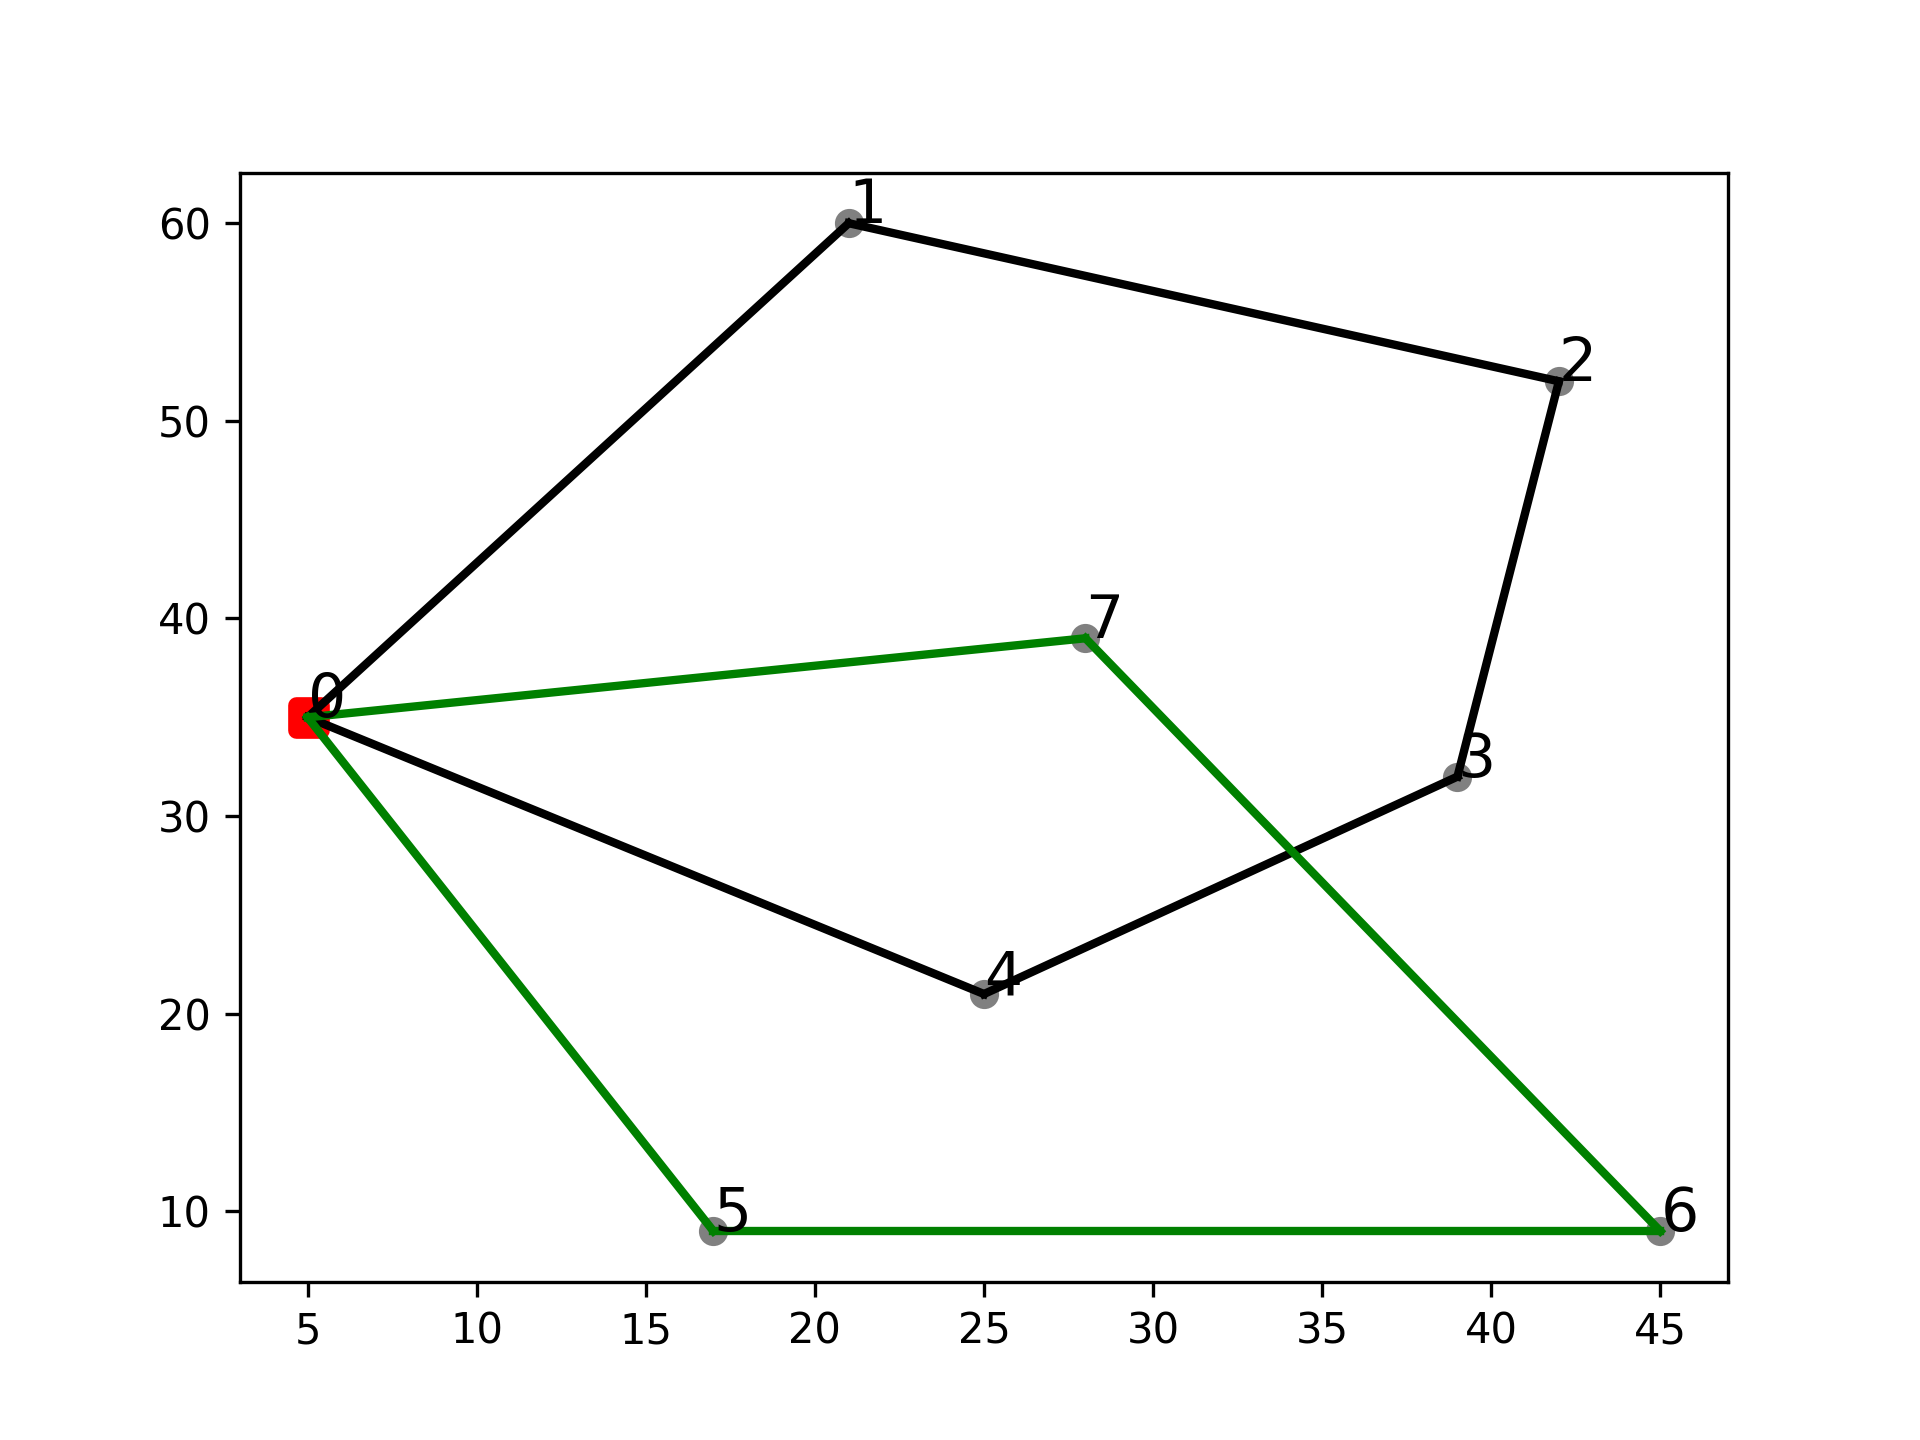
\includegraphics[width=6cm]{resources/opt2/before.png}
    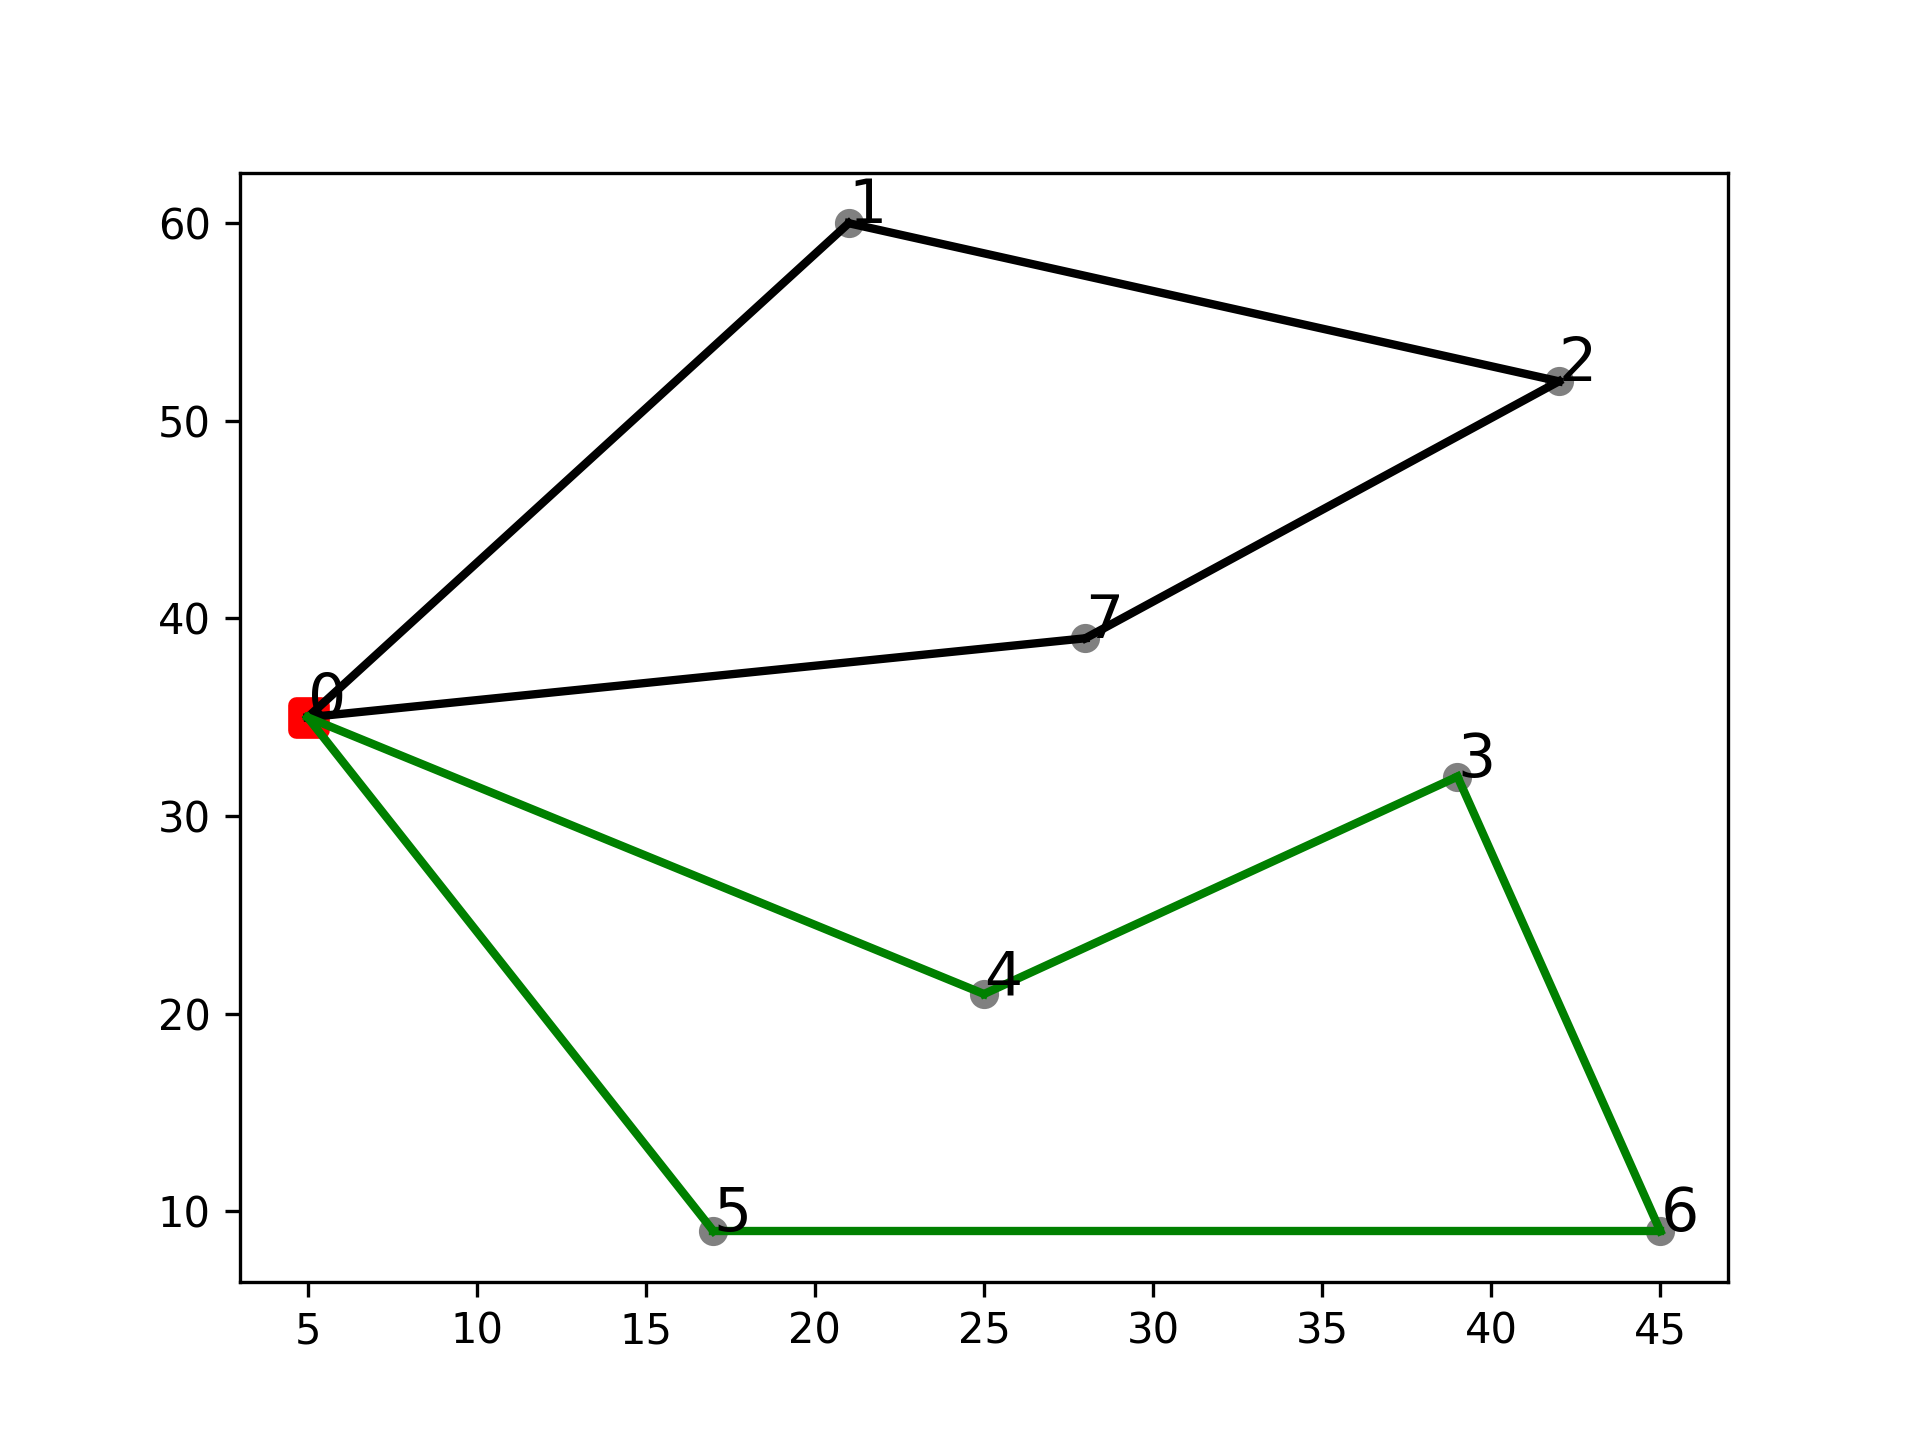
\includegraphics[width=6cm]{resources/opt2/after.png}
    \caption{Ejemplo de intercambio de subrutas. Se intercambia los nodos finales de la ruta negra (3 y 4) a la ruta verde y el nodo final de la ruta verde (7) a la ruta negra.}
    \label{opt2example}
  \end{figure}

  OPT2 logró una mejora en las soluciones respecto a la fase de construcción en todos los casos. Sin embargo habían casos en que esta transformación no era suficiente ya que las soluciones eran parecidas a las óptimas a menos de algunos clientes que debían ser movidos de una ruta a otra u el órden de los clientes dentro de cada ruta.

  \subsubsection*{Insertion}

  Para contemplar algunas falencias de OPT2, se implementó la búsqueda que llamaremos Insertion. Lo que hace es dada dos rutas A y B, intenta insertar un cliente de A en B de manera de reducir la suma de los costos de ambas rutas. El cliente transferido puede quitarse de y ubicarse en cualquier posición mientras las rutas permanezcan factibles.

  \subsection*{Ajuste de parámetros}

  Como se mencionó anteriormente, el ajuste del GRASP se realizó comparando contra las instancias de 25 nodos de Solomon (\ref{solomoninstances}). Los parámetros que se decidió ajustar fueron:

  \begin{enumerate}
    \item {Los que determinan el costo de un movimiento. Estos son los $W_d, W_t y W_w$ de la ecuación \ref{eq:rclmovecost}}.
    \item {En las búsquedas locales, si hacer {\it first improvement} ó {\it best improvement} en cada una y a nivel general. Recordemos que las búsquedas locales implementadas genera vecindades sobre un par de caminos, aquí tenemos un nivel de {\it first/best improvement}. Luego a nivel de solución se puede decidir {\it first/best improvement} para el espacio de búsqueda de pares de caminos, es decir si para el primer par de caminos que $X$ búsqueda local encuentra una mejor solución, o para el par de caminos que mejor solución vecina encuentra.}
  \end{enumerate}

  \subsubsection*{Costo de movimiento}

  Para calibrar los primeros, se consideraron combinaciones de valores de dichos parámetros normalizados a 1 y se ejecutaron todas las instancias de prueba para cada combinación. Los valores considerados fueron 0.0, 0.1, 0.2, 0.3, 0.5, 0.7, 0.9 y 1 para los pesos $W_t$ y $W_d$ y 0.0, 0.1, 0.2, 0.3 y 0.5 para $W_w$. Esto devino en 22 posibles configuraciones que fueron ejecutadas sin incluir la búsqueda local.

  Para la evaluación la mejor asignación de parámetros se tuvieron entonces resultados para 17 instancias de prueba y 22 ejecuciones. El primer paso fué descartar las ejecuciones que no encontraron soluciones factibles para alguna instancia, dado que no hay una fase de corrección de soluciones no factibles, estas configuraciones dejan mal parado al algorítmo. Esto descartó 4 conjuntos de configuraciones.

  Luego, para obtener una visión a grandes rasgos del desempeño de las configuraciones, se decidió comparar la suma del costo y distancia de las 17 soluciones para cada configuración y compararlas en un histograma. De esto, se seleccionó a grosomodo las 7 mejores configuraciones cuyo desempeño agregado es similar como se observa en la figura \ref{cmphistogram}.

  Finalmente, calculando el promedio y desviación estándar del error de las soluciones contra las de referencia, se eligió la configuración que minimizaba ambos valores. Esta es: $W_d = 0.7, W_t = 0.1$ y $W_w = 0.2$.

  \begin{figure}[h!]
    \centering
    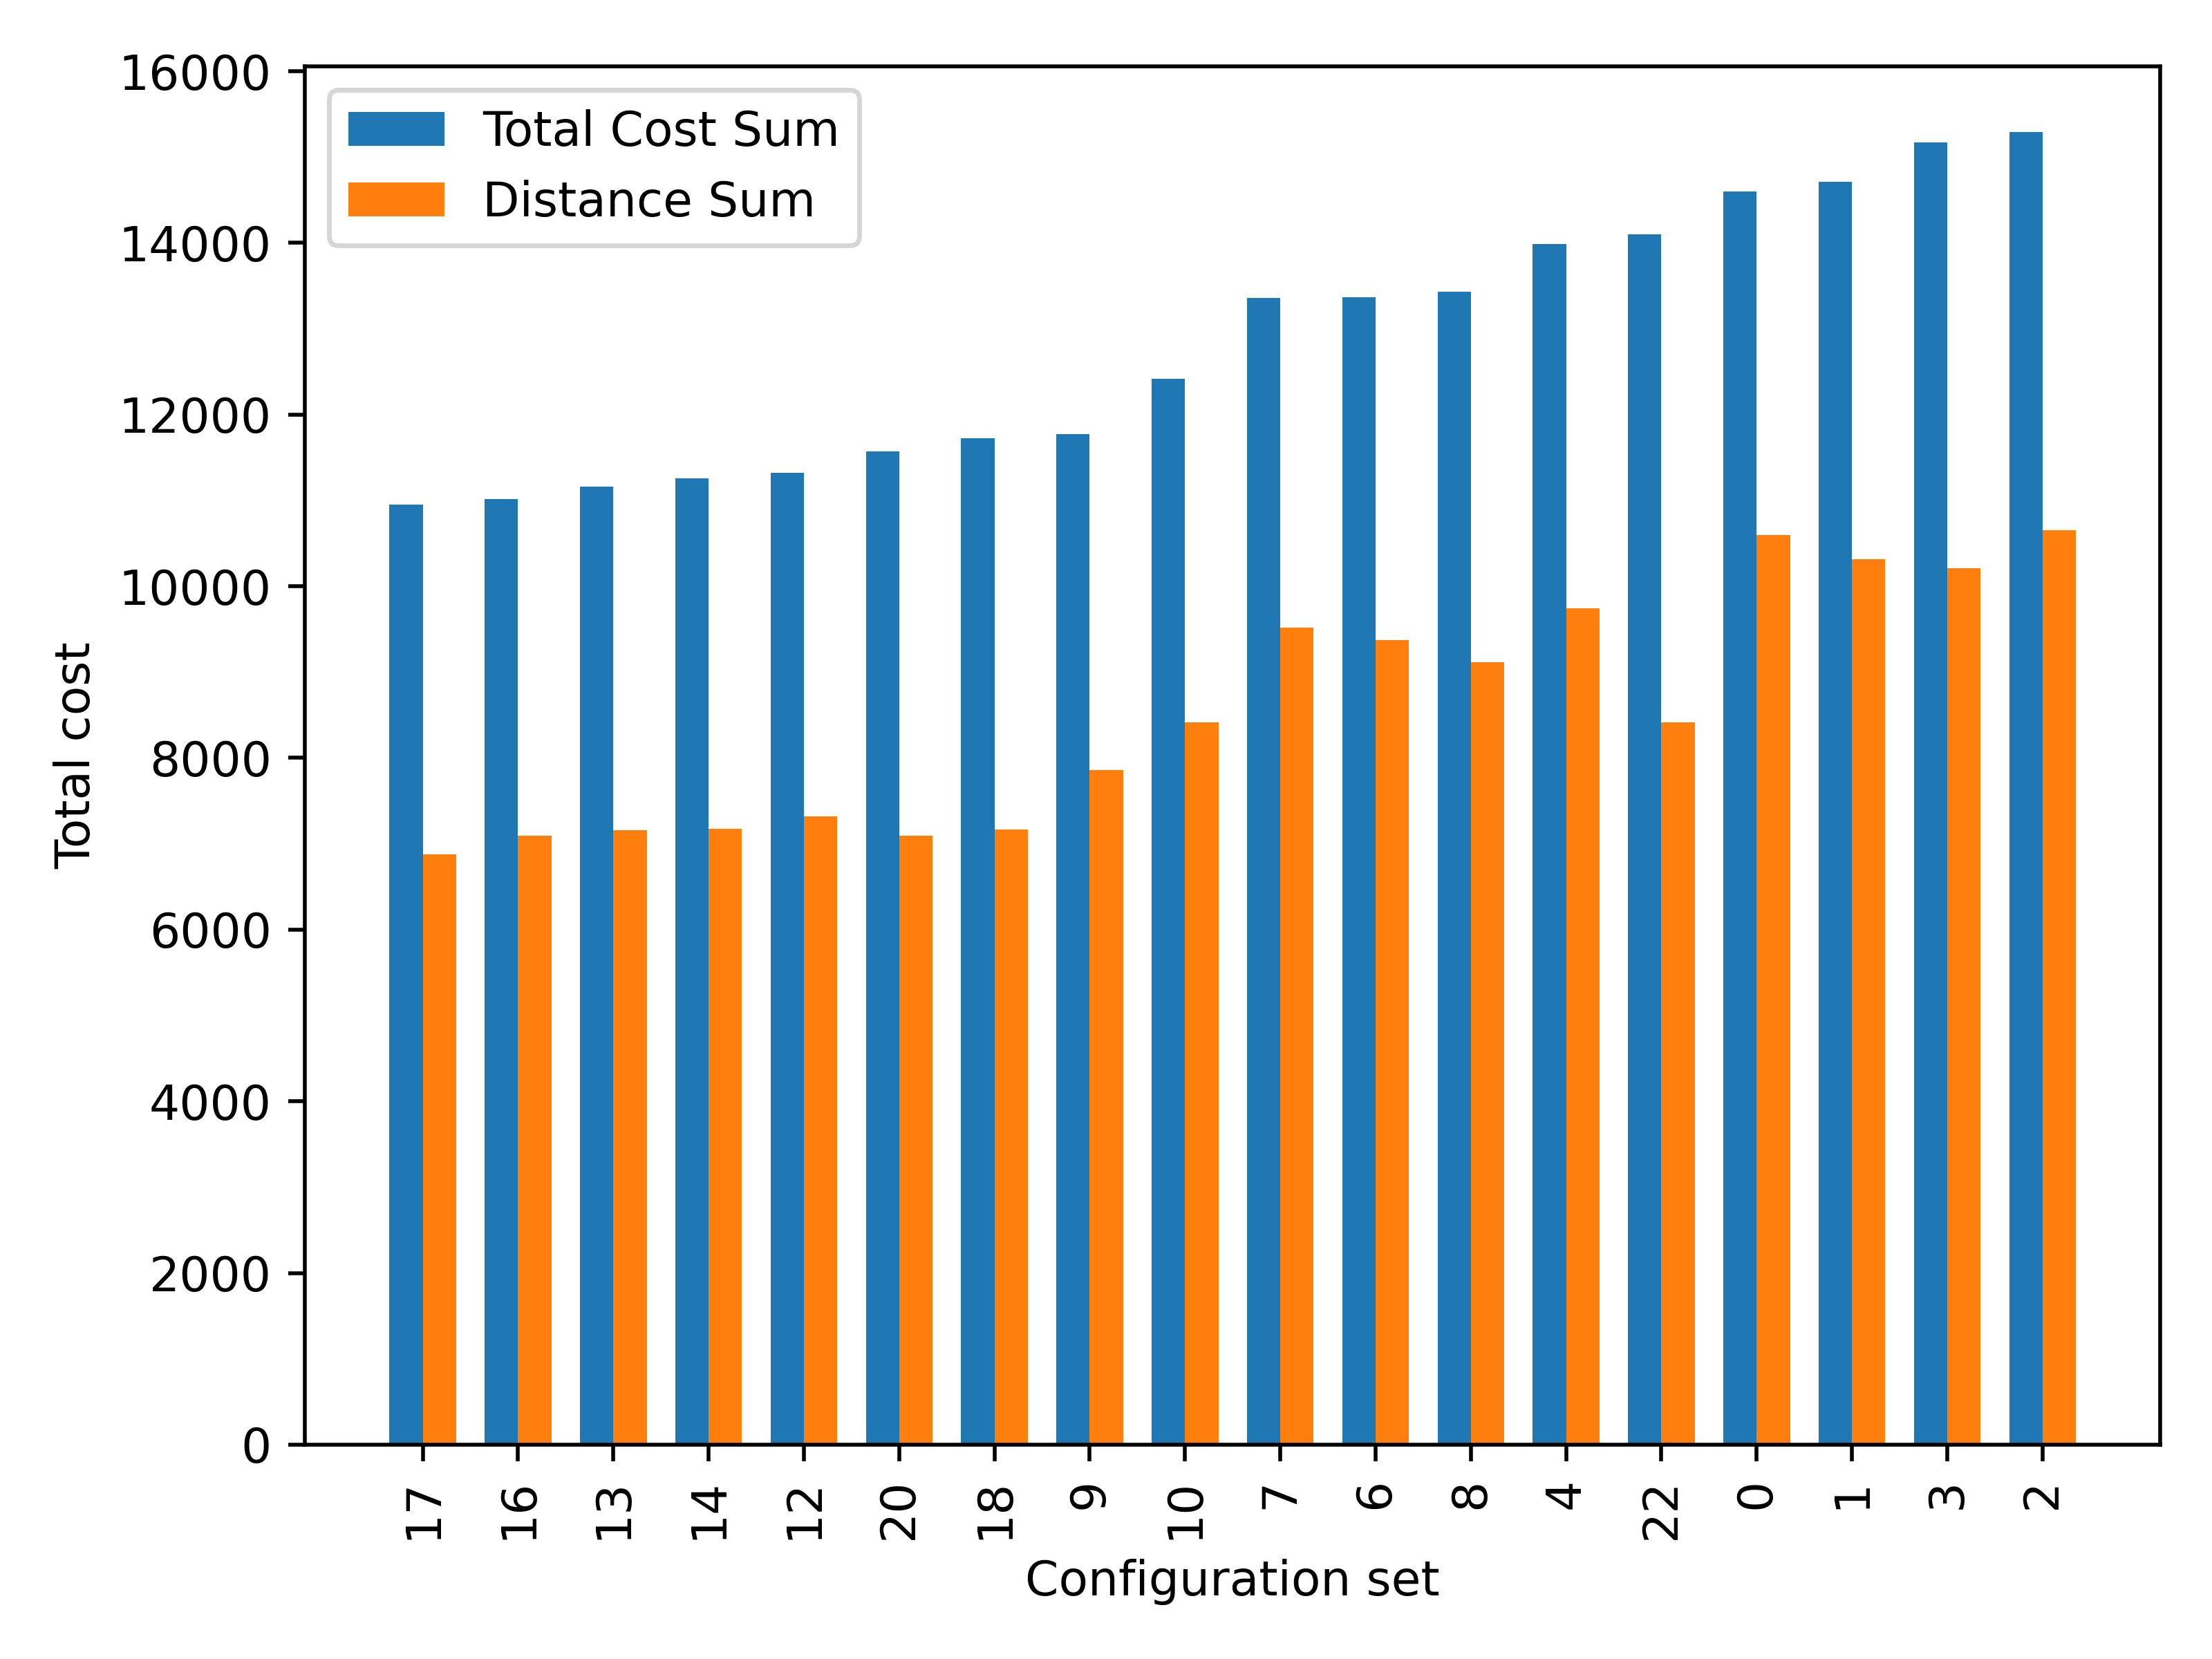
\includegraphics[width=8cm]{resources/tunning/total_cost_histogram_used.png}
    \caption{Histograma donde se compara la suma de los costos de las soluciones encontradas por cada configuración. Se consideran dos factores: el costo total y la distancia. El primero es el valor objetivo, el segundo es un valor que es deseable que sea bajo.}
    \label{cmphistogram}
  \end{figure}

  \subsubsection*{Búsquedas locales}

  Con los parámetros de la sección anterior ya configurados, se procedió a investigar el comportamiento de la búsqueda local respecto a {\it first/best improvement}. Se generaron las ocho combinaciones posibles de los tres parámetros booleanos y se realizaron las ejecuciones tomando $LocalSearchMaxiter = 1000$. Como resultado no se vió mayor diferencia en los resultados de las ejecuciones. Se manejaron tres explicaciones para esto: que el tamaño de las instancias es demasiado chico para notar diferencias; que la cantidad de iteraciones $LocalSearchMaxiter$ haga que {\it best} y {\it first} se comporten igual, es decir que el moverse por la primera mejora reiteradas veces convergiera a la mejor mejora; por último, que la cantidad de vecinos de una solución sean relativamente pocos. Luego de analizar los logs de ejecución utilizando {\it best improvement} en los tres parámetros, se pudo confirmar el último caso. Ocurre que tanto para instancias de 25 nodos como de 100, las vecindades definidas no tienen tamaño mayor a 5 instancias, siendo en promedio entre 1 y 2 vecinos.
  
  Se decidió elegir la configuración mas rápida, es decir {\it first improvement} par los tres parámetros.

  En el cuadro (\ref{table:constructionandlocalsearch}) se observa la mejora de adicionar las búsqueda locales, que pese a definir vecindades chicas logran en general mejorar la solución inicial.

  \begin{table}[h!]
    \centering
    \caption*{{\bf 25 nodos - Construcción y Búsqueda local}}
    \begin{tabular}{ccc}
      \toprule
      Instancia & GRASP Construcción & GRASP Constr. y B. Local \\
      C101.25  &  481.98 & 431.81 \\
      C102.25  &  460.58 & 430.73 \\
      C103.25  &  461.14 & 431.95 \\
      C201.25  &  417.76 & 375.54 \\
      C202.25  &  416.10 & 375.54 \\
      C203.25  &  408.67 & 376.39 \\
      R101.25  & 1275.84 & 1180.6 \\
      R103.25  &  929.49 & 850.55 \\
      R201.25  &  684.08 & 624.70 \\
      R202.25  &  636.86 & 577.12 \\
      R203.25  &  622.20 & 561.72 \\
      RC101.25 &  599.94 & 598.96 \\
      RC102.25 &  600.24 & 575.79 \\
      RC103.25 &  606.67 & 569.08 \\
      RC201.25 &  578.00 & 558.13 \\
      RC202.25 &  546.30 & 512.32 \\
      RC203.25 &  532.91 & 505.49 \\
      
      \midrule
      \bottomrule
    \end{tabular}
    \caption{Comparativa de soluciones obtenidas solo con la fase de construcción contra el agregado de la búsqueda local.}\label{table:constructionandlocalsearch}
  \end{table}

  \section*{Resultados}

  Luego de calibrar un poco el algorítmo, se realizaron pruebas con instancias de 100 nodos para algunas de las cuales existen resultados exactos en caso de ventana fija. En el cuadro (\ref{table:res100nodesfixed}) se comparan los resultados de ventana fija contra los óptimos o mejores soluciones encontradas provistas por Solomon (\ref{solomoninstances}). Luego en los cuadros (\ref{table:res100nodesflexibledistance}) y (\ref{table:res100nodesflexiblecost}) se comparan los resultados de GRASP ventana fija vs GRASP ventana flexible considerando la distancia en el primer caso y el costo en el segundo.
  
  También se detallan los resultados de la ejecución en las instancias de 25 nodos en los cuadros (\ref{table:res25nodesfixed}) para ventana fija y (\ref{table:res25nodesflexible}) para ventana flexible, comparando contra las los mejores valores de soluciones que se encuentran disponibles.

  La configuración de las ejecuciones del GRASP fueron $500000$ iteraciones para las instancias de 25 nodos y $100000$ para las de 100, con $20$ hilos de ejecución y un parámetro $\alpha$ de la RCL de $0.8$. El tiempo de ejecución del el conjunto de instancias de 25 nodos rondó en las 3 horas y de las de 100 nodos en 10 horas.

  Las instancias con ventana flexible tienen un factor $w = 0.5$ y $\rho = 0.1$. Todas las instancias tienen flota homogénea.

  \begin{table}[h!]
    \centering
    \caption*{{\bf 100 nodos - Ventana Fija}}
    \begin{tabular}{ccccc}
      \toprule
      Instancia & Óptimo & Mejor conocido & GRASP V. Fija & Dif. (\%) \\
      \midrule
      C101.100  & 827.3  &       - & 828.936 &  0.20 \\
      C201.100  & 589.1  &       - & 591.556 &  0.42 \\
      R101.100  & 1637.7 &       - & 1739.40 &  6.21 \\
      R108.100  &      - &  960.88 & 1050.03 &  9.28 \\
      R201.100  & 1143.2 &       - & 1287.16 & 12.59 \\
      R208.100  &      - &  726.75 & 790.434 &  8.76 \\ 
      RC101.100 & 1619.8 &       - & 1771.28 &  9.35 \\
      RC104.100 &      - & 1135.48 & 1287.30 & 13.37 \\
      RC201.100 & 1261.8 &       - & 1547.04 & 22.61 \\
      RC204.100 &      - &  798.41 & 1162.66 & 45.62 \\
      \bottomrule
    \end{tabular}
    \caption{Resultados de la ejecución de las algunas instancias de 100 nodos con ventana fija comparando la distancia de la soluciones contra el óptimo o mejor conocido en (\ref{solomoninstances}). Unicamente dos de las soluciones fueron muy cercanos al óptimo. Probablemente con un tiempo mayor de ejecución se obtengan mejores resultados.}\label{table:res100nodesfixed}.
  \end{table}

  \begin{table}[h!]
    \centering
    \caption*{{\bf 100 nodos - Distancia Ventana Flexible}}
    \begin{tabular}{ccccc}
      \toprule
      Instancia & GRASP V. Fija & GRASP V. Flexible & Dif. (\%) \\
      \midrule
      C101.100  & 828.936 &  860.33 &   3.65 \\
      C201.100  & 591.556 &  607.13 &   2.57 \\
      R101.100  & 1739.40 & 1603.61 &  -8.47 \\
      R108.100  & 1050.03 &  990.71 &  -5.99 \\
      R201.100  & 1287.16 & 1267.35 &  -1.56 \\
      R208.100  & 790.434 &  784.01 &  -0.82 \\ 
      RC101.100 & 1771.28 & 1597.98 & -10.84 \\
      RC104.100 & 1287.30 & 1166.60 & -10.35 \\
      RC201.100 & 1547.04 & 1465.57 &  -5.56 \\
      RC204.100 & 1162.66 & 1151.39 &  -0.98 \\
      \bottomrule
    \end{tabular}
    \caption{Comparativa entre distancia de la soluciones obtenidas por el GRASP con y sin ventana flexible.}\label{table:res100nodesflexibledistance}
  \end{table}

  \begin{table}[h!]
    \centering
    \caption*{{\bf 100 nodos - Costo Ventana Flexible}}
    \begin{tabular}{ccccc}
      \toprule
      Instancia & GRASP V. Fija & GRASP V. Flexible & Dif. (\%) \\
      \midrule
      C101.100  & 1868.93 & 1820.33 &  -2.67 \\
      C201.100  &  911.55 &  927.13 &   1.68 \\
      R101.100  & 3419.40 & 3203.61 &  -6.74 \\
      R108.100  & 2010.03 & 1630.71 & -23.26 \\
      R201.100  & 1687.57 & 1587.35 &  -6.31 \\
      R208.100  & 1110.43 & 1024.01 &  -8.44 \\ 
      RC101.100 & 3211.28 & 2877.98 & -11.58 \\
      RC104.100 & 2247.30 & 1966.60 & -14.27 \\
      RC201.100 & 2347.04 & 2265.57 &  -3.60 \\
      RC204.100 & 1882.66 & 1871.39 &  -0.60 \\
      \bottomrule
    \end{tabular}
    \caption{Comparativa entre costos de la soluciones obtenidas por el GRASP con y sin ventana flexible. Si contrastamos la columna de diferencia contra el cuadro comparativo de distancias (\ref{table:res100nodesflexibledistance}), se puede observar que las soluciones con ventana flexible sacan mayor ventaja al comparar el costo. Esto se explica porque al aumentar el tamaño de las ventanas, el algorítmo puede satisfacer más clientes con menos vehículos con la consecuencia de aumentar la distancia recorrida pero incurriendo en un menor costo fijo total.}\label{table:res100nodesflexiblecost}
  \end{table}

  \begin{table}[h!]
    \centering
    \caption*{{\bf 25 nodos - Ventana fija}}
    \begin{tabular}{cccc}
      \toprule
      Instancia & Óptimo & Solución GRASP & Error (\%) \\
      C101.25  & 191.3 & 191.81 &  0.27 \\
      C102.25  & 190.3 & 190.73 &  0.23 \\
      C103.25  & 190.3 & 194.26 &  2.08 \\
      C201.25  & 214.7 & 215.54 &  0.39 \\
      C202.25  & 214.7 & 215.54 &  0.39 \\
      C203.25  & 214.7 & 215.54 &  0.39 \\
      R101.25  & 617.1 & 618.32 &  0.20 \\
      R103.25  & 454.6 & 484.58 &  6.60 \\
      R201.25  & 463.3 & 523.65 &  13.03 \\
      R202.25  & 410.5 & 458.96 &  11.81 \\
      R203.25  & 391.4 & 405.00 &  3.48 \\
      RC101.25 & 461.1 & 462.15 &  0.23 \\
      RC102.25 & 351.8 & 357.76 &  1.70 \\
      RC103.25 & 332.8 & 338.73 &  1.78 \\
      RC201.25 & 360.2 & 432.29 &  20.02 \\
      RC202.25 & 338   & 377.14 &  11.58 \\
      RC203.25 & 326.9 & 356.21 &  8.97 \\
      \midrule
      \bottomrule
    \end{tabular}
    \caption{Comparativa de resultados contra el óptimo. En este caso el valor de la solución es la distancia total de los recorridos. Las soluciones óptimas de Solomon (\ref{solomoninstances}) están expresadas en esta unidad.}\label{table:res25nodesfixed}
  \end{table}

  \begin{table}[h!]
    \centering
    \caption*{{\bf 25 nodos - Ventana flexible}}
    \begin{tabular}{cccc}
      \toprule
      Instancia & Mejor Solución & Solución GRASP & Error (\%) \\
      \midrule
      C101.25  &  431.7	 & 431.81 &	0.03  \\
      C102.25  &  430.6	 & 430.73 &	0.03 \\
      C103.25  &  430.6	 & 431.95 &	0.31 \\
      C201.25  &  375.6	 & 375.54 &	-0.02 \\
      C202.25  &  303.4	 & 375.54 &	23.78 \\
      C203.25  &  303.4	 & 376.39 &	24.06 \\
      R101.25  &  1167.2 & 1180.6 &  1.15 \\
      R103.25  &  771.51 & 850.55 &	10.25 \\
      R201.25  &  639.5	 & 624.70 &	-2.31 \\
      R202.25  &  555.5	 & 577.12 &	3.89 \\
      R203.25  &  560.8	 & 561.72 &	0.17 \\
      RC101.25 &  600.7	 & 598.96 &	-0.29 \\
      RC102.25 &  574	   & 575.79 &	0.31 \\
      RC103.25 &  567.1	 & 569.08 &	0.35 \\
      RC201.25 &  565.9	 & 558.13 &	-1.37 \\
      RC202.25 &  516.2	 & 512.32 &	-0.75 \\
      RC203.25 &  517.2	 & 505.49 &	-2.26 \\
      \bottomrule
    \end{tabular}
    \caption{Comparativa de resultados con ventana flexible contra los provistos por (\ref{inco}). El valor de las soluciones en este caso es la suma de costos fijos y costos variables de los vehículos. A excepción de dos instancias, los resultados parecen ser muy buenos e incluso superando en las últimas filas.}\label{table:res25nodesflexible}
  \end{table}

  \section*{Conclusión}

  Se concluye que el la metaheurístca implementada se desempeña correctamente y es suficientemente configurable para sacar buen provecho de ella con algún trabajo adicional de análisis sobre los parámetros.

  \section*{Trabajo a futuro}

  \subsection*{Mejor consideración de movimientos por vehículo}
  
  En la implementación de este trabajo, la cantidad de movimientos por vehículo a incluir en la RCL está dada por el parámetro $MovesPerVehicle$. Se podría tomar enfoque mas inteligente y considerar una cantidad variable de movimientos dependiendo que tan buenos sean estos, por ejemplo, con un parámetro $\alpha$, similar a la forma en que se construye la RCL.

  \subsection*{Mejor calibración del GRASP}

  En este trabajo se mencionó la calibración de algunos parámetros pero el algorítmo implementado tiene algunos más que puede ser útil investigar. Algunos de estos son: el $\alpha$ de la RCL; $MovesPerVehicle$; y $MaxWaitTime$ utilizado para descartar soluciones durante la construcción que superan dicho tiempo de espera, un valor bajo de este parámetro puede reducir drásticamente los movimientos considerados, por ejemplo, Solomon (\ref{solomon}) considera los valores 30, 60 y 120.

  \subsection*{Ejecuciones de mayor escala}

  Las ejecuciones consideradas en este trabajo rondan en el orden de horas y utilizan 20 núcleos de CPU, se podrían considerar ejecuciones con limites mucho mayores de tiempo y posiblemente abarcar un mayor espacio de búsqueda.

  \subsection*{Detención temprana}

  Como manera de ahorrar tiempo de ejecución se puede implementar un mecanismo de detención temprana, por ejemplo, si no se ha mejorado la solución en $X$ iteraciones.

  \section*{Implementación}

  La implementación del GRASP y programas utilitarios se encuentra en el repositorio público (\ref{repo}). Se utilizó el lenguaje Rust para el GRASP puntualmente ya que es un lenguaje compilado de buen desempeño y python para procesamiento de los resultados.

  Las instrucciones de ejecución del GRASP principal se detallan en el repositorio. Luego se proveen alguns scripts python:
  \begin{description}
    \item[summarize.py]: Script que dados varios archivos con soluciones, genera un csv con los principales aspectos de las soluciones: costo total, distancia, cantidad de vehículos, nombre de la instancia.
    \item[validate.py]: Script que valida un archivo de solución. Utilizado principalmente durante el desarrollo para asegurarse que las soluciones generadas sean factibles.
    \item[draw.py]: Script que dibuja las rutas dado un archivo solución.
  \end{description}

  El GRASP puede ejecutar de forma paralela utilizando hilos del sistema operativo. La ejecución paralela ejecuta varias instancias de GRASP y al final toma la mejor solución de todas las instancias.

  \section*{Referencias}

  \begin{enumerate}
    \item{\label{jiang} Jun Jiang, Kien Ming Ng, Kim Leng Poh, Kwong Meng Teo (2014). Vehicle routing problem with a heterogeneous fleet and time windows}
    \item{\label{inco} Lucía Barrero, Rodrigo Viera, Franco Robledo, Claudio Risso, Sergio Nesmachnow, Andrei Tchernykh (2020). Exact resolution of the Vehicle Routing Problem with Flexible Time Windows}
    \item{\label{solomon} Solomon, M. M. (1985). Algorithms for the vehicle routing and scheduling problems with time window constraints}
    \item{\label{solomoninstances} Solomon, M. M. VRPTW Benchmark Problems \url{http://w.cba.neu.edu/~msolomon/problems.htm}}
    \item{\label{repo} Repositorio de la implementación del GRASP. \url{https://github.com/joaquinco/mor-proj}}
  \end{enumerate}
\end{document}
